\title{Semantics of Functional Programming}
\subtitle{\PCF{} and its Operational Semantics}
\author[L.-T. Chen]{Chen, Liang-Ting\\
  \href{mailto:lxc@iis.sinica.edu.tw}{\texttt{lxc@iis.sinica.edu.tw}}}
\institute[IIS, Sinica]{Institute of Information Science, Academia Sinica}
\begin{document}

\setcounter{framenumber}{-1}

\frame{\maketitle}

\begin{frame}[c]
  \frametitle{Why semantics?}
  \begin{quotation}
    The hitch is that defining a language \emph{a posteriori}, i.e.\ after its
    design has been frozen by the existence of implementations and uses, can
    hardly improve it.  To create a good programming language, semantics must
    be used \emph{a priori}, as a design tool that embodies and extends the
    intuitive notion of uniformity. \\~\\
    \hfill --- \textrm{John C.\ Reynolds}
  \end{quotation}
\end{frame}

\begin{frame}[c]
  \frametitle{\protect\textbf{C\textplus\textplus}}
  \begin{itemize}
      \item Implementation-led design.
      \item \emph{\textbf{C\textplus\textplus} The International Standard},
        \alert{1338~pp.}, 2012. \\
        Note that the committee consists of \alert{200\textplus{} people}.
      \item \alert{1900\textplus} language issues!
  \end{itemize}
  \begin{center}
    \only<presentation>{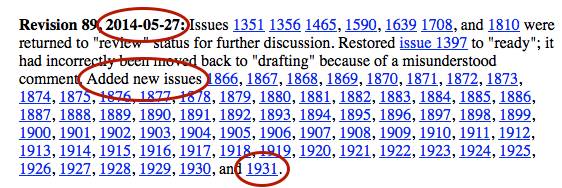
\includegraphics[scale=.5]{C++issues.png}}
  \end{center}
\end{frame}

\begin{frame}[c]
  \frametitle{\protect\textbf{Standard ML}}
  \begin{itemize}
    \item Semantics-led design.
    \item R.\ Milner, M.\ Tofte, R.\ Harper, and D.\ MacQueen \emph{The Definition of
        \textbf{Standard ML} (Revised)}, \alert{128~pp.}, 1997. \\
    \item Standard ML is a safe, modular, strict, functional, polymorphic
      programming language \dots and \alert{a formal definition with a proof of
        soundness}.
  \end{itemize}
\end{frame}

\begin{frame}{Overview}
  In this lecture, we will present simply typed lambda calculus 
  in a different manner, where terms and typing rules are introduced
  separately. In this approach, terms might not be well-typed at all.
  \\~\\

  Then, we discuss its computational meaning by \textbf{one-step reduction} and
  define many-step reduction.  Later we introduce the concept of
  \textbf{type safety}. 
  \\~\\

  Finally, we extend simply typed lambda calculus with natural numbers
  and general recursion. This extension is called \PCF{}, \emph{Programming
    Computable Functional}. We formalise new features
  by what we have learnt later.
\end{frame}

\section{Simply typed lambda calculus {\`{a} la} Curry}
\begin{frame}{The approach \emph{\`{a} la} Curry}
  We introduce a different approach to simply typed lambda calculus where
  terms and typing rules are introduced separately.
  \\~\\
    
  \begin{columns}
    \column{.5\textwidth}
    \begin{prooftree}
    \AXC{$x\;\,\var$}
    \UIC{$x\;\,\term\vphantom{\Gamma, x : \sigma, \Delta \vdash x : \sigma}$}
    \end{prooftree}

    \column{.5\textwidth}
    \begin{prooftree}
    \AXC{$\vphantom{x\;\,\var}$}
    \RightLabel{(var)} \UIC{$\Gamma, x :
      \sigma, \Delta \vdash x : \sigma$}
    \end{prooftree}
  \end{columns}

  \begin{columns}
    \column{.5\textwidth}
    \begin{prooftree}
      \AXC{$x \;\,\var$} \AXC{$\M \;\, \term\vphantom{\Gamma, x : \sigma \vdash
          \M : \tau}$}
      \BIC{$\lambda \alert{x.\, \M} \;\,\term
      \vphantom{\Gamma \vdash \lambda x .\, \M : \sigma \to \tau}$} 
    \end{prooftree}

    \column{.5\textwidth}
    \begin{prooftree}
      \AXC{$\Gamma, x : \sigma \vdash \M : \tau$}
      \RightLabel{(abs)}
      \UIC{$\Gamma \vdash \lambda x .\, \M : \sigma \to \tau$} 
    \end{prooftree}
  \end{columns}

  \begin{columns}
    \column{.5\textwidth}
    \begin{prooftree}
      \AXC{$\M\;\,\term$} \AXC{$\N\;\,\term \vphantom{\Gamma \vdash \M : \sigma
          \to \tau}$}
      \BIC{$\M\;\N\;\,\term
      \vphantom{\Gamma \vdash \M\; \N : \tau}$}
    \end{prooftree}

    \column{.5\textwidth}
    \begin{prooftree}
      \AXC{$\Gamma \vdash \M : \sigma \to \tau$} \AXC{$\Gamma \vdash \N :
      \sigma$}
    \RightLabel{(app)}
    \BIC{$\Gamma \vdash \M\; \N : \tau$}
    \end{prooftree}
  \end{columns}
\end{frame}

\begin{frame}{The existence of ill-typed terms}
  In contrast the approach \emph{\`{a} la} Church where every term is
  introduced with a type, there are ill-typed terms in the approach
  \emph{\`{a} la} Curry:
  \\~\\
      \begin{example}
        $(\lambda x.\,x\;x)$ is a term if~$x$ is a variable,
        because
        \begin{prooftree}
          \AXC{$x\;\,\var$}
          \AXC{$x\;\,\var$}
          \UIC{$x\;\,\term$}
          \AXC{$x\;\,\var$}
          \UIC{$x\;\,\term$}
          \BIC{$x\;x\;\,\term$}
          \BIC{$\lambda x.\, x\;x\;\,\term$}
        \end{prooftree}
      \end{example}
      ~\\
   However, $(\lambda x.\, x\;x)$ cannot be assigned a type
   unless $\sigma \to \sigma = \sigma$.
\end{frame}

\begin{frame}{Reduction}
  \textbf{One-step reduction} relation~$\leadsto$ between
  terms is introduced to describe the flow of computation from a term to
  another term in a single step, regardless of types. We introduce two rules
  for applications:  \\~\\
    \begin{prooftree}
      \AXC{$\M \leadsto \M'$}
      \RightLabel{($\leadsto$-lapp)}
      \UIC{$\M\;\N \leadsto \M'\;\N$}
    \end{prooftree}
    \begin{prooftree}
      \AXC{}
      \RightLabel{($\leadsto$-app)}
      \UIC{$(\lambda x .\, \M)\; \N \leadsto
        \M[\N/x] $}
    \end{prooftree}
    ~\\
  \only<article>{
      These two rules formalise what we call \emph{call-by-name}
      evaluation strategy, where its arguments are evaluated only if used at
      least once. This allows us to feed a non-terminating argument and produce
      a terminating result.

      In most of programming languages such as \textbf{C}, arguments are
      evaluated to values before applications, and this evaluation strategy is
      called \emph{call-by-value}.  }
  \begin{example}
  $ (\lambda x.\, \lambda y.\,x)\;\M\;\N$ can reduce to~$\M$
  by the following derivation
  \begin{prooftree}
    \AXC{}
    \RightLabel{($\leadsto$-app)}
    \UIC{$(\lambda x.\, \lambda y.\, x)\;\M \leadsto
      (\lambda y.\,\M)$}
    \RightLabel{($\leadsto$-lapp)}
    \UIC{$((\lambda x.\, \lambda y.\, x)\;\M)\;\N
      \leadsto (\lambda y.\,\M)\; \N$}
  \end{prooftree}
\end{example}
\end{frame}

\begin{frame}{Many-step reduction}
  As we will mostly discuss a sequence of reductions, it is convenient to
  define another relation~$\leadsto^*$ so that $\M \leadsto^* \N$ means $\M$
  reduces to~$\N$ in finitely many steps. 
  \\~\\
  \begin{definition}
    The many-step reduction relation~$\leadsto^*$ is defined inductively by 
    \begin{center}
    \begin{tabular}[c]{c c}
      \AXC{$\vphantom{\M_2 \leadsto^* \M_3}$}
      \UIC{$\M \leadsto^* \M$}
      \DP & 
      \AXC{$\M_1 \leadsto \M_2$}
      \AXC{$\M_2 \leadsto^* \M_3$}
      \insertBetweenHyps{\hskip .5em}
      \BIC{$\M_1 \leadsto^* \M_3$}
      \DP
    \end{tabular}
  \end{center}
  \end{definition}
  ~\\
  \begin{proposition}[Reflexivity of $\leadsto^*$]
    For every term $\M$, $\M \leadsto^* \M$. 
  \end{proposition}
\end{frame}

\begin{frame}
  For example, one has
  \[
    (\lambda x.\, \lambda y.\, x)\; \M\;\N \leadsto^*
    (\lambda y.\, \M)\; \N
  \]
  by the derivation 
  \begin{prooftree}
    \AXC{}
    \UIC{$(\lambda x.\, \lambda y.\, x)\;\M \leadsto (\lambda y.\, \M)$}
    \UIC{$((\lambda x.\, \lambda y.\, x)\;\M)\;\N
      \leadsto (\lambda y.\,\M)\; \N$}
    \insertBetweenHyps{\hskip -2pt}
    \AXC{$(\lambda y.\,\M)\;\N \leadsto^* (\lambda y.\,\M)\;\N$}
    \BIC{$(\lambda x.\, y.\, x)\;\M\;\N \leadsto^* (\lambda y.\,\M)\;\N$}
  \end{prooftree}
  ~\\
  
  \textbf{Exercise}. Evaluate the following terms (formally or
  informally). 
  \begin{enumerate}
    \item $(\lambda x.\, x)\;y$
    \item $(\lambda x.\, x\;x)\;(\lambda x.\, x\;x)$
    \item $(\lambda x.\,\lambda y.\,\lambda z.\, y)\;\M_0\;\M_1\;\M_2$
  \end{enumerate}
\end{frame}

\begin{frame}{Induction on derivation}
  Every instance of $\M \leadsto^* \N$ must be constructed by one of the cases, so
  we can analyse its structure case by case. 
  \\~\\
  \begin{proposition}[Transitivity of $\leadsto^*$]
    For every three terms $\M_1$, $\M_2$, and $\M_3$, if $\M_1 \leadsto^* \M_2$
    and $\M_2 \leadsto^* \M_3$, then $\M_1 \leadsto^* \M_3$.
  \end{proposition}
  ~\\
  Given derivations of $\M_1 \leadsto^* \M_2$ and $\M_2 \leadsto^* \M_3$,
  we do case analysis on the derivation of $\M_1 \leadsto^* \M_2$. 
  Also, we can assume that the premise satisfy this property, that is, the
  induction hypothesis. 
\end{frame}

\begin{frame}
  \begin{proof}
    \begin{enumerate}
      \item For \AXC{} \UIC{$\M_1 \leadsto^* \M_1$} \DP, it unifies
        $\M_2$ to~$\M_1$, so the given derivation $\M_2 \leadsto^* \M_3$
        is just the goal derivation as $\M_1 = \M_2$. 
        ~\\
      \item For \AXC{$\M_1 \leadsto \M$}\AXC{$\M \leadsto^* \M_2$}
        \BIC{$\M_1 \leadsto^* \M_2$}\DP, 
        we infer that $\M \leadsto^* \M_3$ by induction hypothesis, so we
        derive the goal
        \begin{prooftree}
          \AXC{$\M_1 \leadsto \M$}
          \AXC{$\M \leadsto^* \M_3$}
          \BIC{$\M_1 \leadsto^* \M_3$}
        \end{prooftree}
    \end{enumerate}
  \end{proof}
  ~\\

  Similarly, we can do induction on the formation of terms, typing rules,
  and any other inductive definitions. 
  \\~\\

  \textbf{Exercise.} Show that if $\M \leadsto^* \M'$ then
  $\M\;\N \leadsto^* \M'\;\N$ for any term~$\N$ by induction on
  the derivation of~$\M \leadsto^* \M'$. 
\end{frame}


\begin{frame}{Type safety: well-typed programs don't go wrong}
  Well-typed closed terms have some nice properties.  First, every well-typed
  closed term can reduce further or it is a \alert{value}.
  \\~\\
  \begin{theorem}[Progress Theorem]
    If ${}\vdash \M:\tau$, then either $\M \leadsto \M'$ for some~$\M'$
    or $\M = \lambda x.\, \M'$. 
  \end{theorem}
  ~\\
  To show this property, we do structural induction on the derivation
  of~${}\vdash \M : \tau$ and either produce a derivation of~$\M \leadsto \M'$
  or show that $\M = \lambda x.\, \M'$.
\end{frame}

\begin{frame}
  \begin{proof}
    \begin{enumerate}
      \item The context of 
        \AXC{}\UIC{$\Gamma, x : \sigma, \Delta \vdash x : \sigma$}\DP, 
        is non-empty, so it does not satisfy the assumption.
      \item For that case \AXC{$x : \sigma\vdash \M : \tau$}
        \RightLabel{(abs)}
        \UIC{${}\vdash \lambda x.\, \M : \sigma \to \tau$}\DP, 
         we have already given a term in this form $\lambda x.\, \M$. 
         \\~\\
       \item For \AXC{${}\vdash \M : \sigma\to\tau$}\AXC{${}\vdash \N :
           \sigma$}\RightLabel{(app)}\BIC{${}\vdash \M\;\N : \tau$}\DP, 
         by introduction hypothesis either $\M \leadsto \M'$ for some~$\M'$
         or $\M = \lambda x.\, \M'$. For the former case, we apply
         ($\leadsto$-lapp):
         \begin{prooftree}
           \AXC{$\M \leadsto \M'$}
           \UIC{$\M\;\N\leadsto \M'\;\N$}
         \end{prooftree}
         ~\\
         For the latter case, we apply ($\leadsto$-app)
         \begin{prooftree}
           \AXC{}
           \UIC{$(\lambda x. \, \M')\;\N \leadsto \M'[\N/x]$}
         \end{prooftree}
    \end{enumerate}
  \end{proof}
\end{frame}

\begin{frame}
  Moreover, the type of a well-typed closed term is always preserved by reductions:
  \\~\\
  \begin{theorem}[Preservation Theorem]
    If ${}\vdash \M:\tau$ and $\M \leadsto \M'$, then ${}\vdash \M':\tau$.  
  \end{theorem}
  ~\\
  However, to show this property, we need the following lemma saying that
  types are preserved by substitution.
  \\~\\
  \begin{lemma}[Substitution Lemma]
    If $\Gamma, x : \sigma \vdash \alert{\M : \tau}$
    and $\Gamma \vdash \N : \sigma$,
    then $\Gamma \vdash \alert{\M[\N/x] : \tau}$.
  \end{lemma}
\end{frame}

\begin{frame}
  By the introduction on the derivation of ${}\vdash \M : \tau$
  and $\M \leadsto \M'$ at the same time. 
  \\~\\
  \begin{proof}[Proof of Preservation Theorem]
    \begin{enumerate}
      \item ${}\vdash \M : \tau$ cannot be constructed by $(var)$, since the
        context is empty. 
        \\~\\
      \item For \AXC{$x : \sigma \vdash \M : \tau$}
        \UIC{${}\vdash \lambda x.\, \M : \sigma \to \tau$}\DP, there is no
        reduction rule for~$\lambda x.\, \M$, so a derivation~$(\lambda x.\,\M)
        \leadsto \M'$ cannot exist. 
        \\~\\
      \item For \AXC{${}\vdash \M : \sigma \to \tau$}
        \AXC{${}\vdash \N : \sigma$}\BIC{${}\vdash \M\;\N : \tau$}\DP, 
        we do induction on the derivation of $\M\;\N \leadsto \M'$. 
    \end{enumerate}
  \end{proof}
\end{frame}

\begin{frame}{Reductions on ill-typed terms}
  Reductions can be applied to ill-typed terms
  and it reduces to a well-typed closed term! 
  \[
        (\lambda x.\,\lambda y.\,x)\;(\lambda x.\,x)\;(\lambda x.\,x\;x)
        \leadsto^* (\lambda x.\, x)
  \]
  ~\\

  On the other hand, 
  the reduction of ill-typed terms may not reduce to a value at all
  \begin{align*}
    x\; x \not\leadsto
  \end{align*}
\end{frame}

\begin{frame}{Summary}
  To define a language, we specify following sets of rules 
  \begin{description}[Semantics]
    \item[Syntax] type, term, and typing rules. 
    \item[Semantics] reduction rules.
  \end{description}
  ~\\
  In particular, well-typed closed terms share type safety:
  \\~\\
  \begin{description}[Preservation Theorem]
    \item[Progress Theorem] for every well-typed closed term, it either can 
      reduce further or is a value;
    \item[Preservation Theorem] 
      for every well-typed closed term, its type is preserved by reduction. 
  \end{description}
  ~\\

  Next, we add some features to simply typed lambda calculus
  and type safety remains. 
\end{frame}
\section{Programming with typed recursion}
\begin{frame}{Introduction to \PCF}
  \PCF{}, which stands for \textbf{Programming Computable Functionals}, is a
  functional programming language and it consists of
  \begin{enumerate}
    \item simply typed lambda calculus,
    \item natural numbers, and
    \item general recursion (to be explained). 
  \end{enumerate}
  We will introduce the latter two features step by step.
  \\~\\

  It has two rules of type formation:
    \begin{columns}[t]
      \column{.5\textwidth}
      \begin{prooftree}
        \AXC{$\vphantom{\tau_1\;\,\type}$}
        \UIC{$\nat\;\,\type$}
      \end{prooftree}
      \column{.5\textwidth}
      \begin{prooftree}
        \AXC{$\tau_1\;\,\type$}
        \AXC{$\tau_2 \;\,\type$}
        \BIC{$\tau_1 \to \tau_2 \;\,\type$}
      \end{prooftree}
    \end{columns}
    ~\\

    Still, `set' is a synonyms of `type'. 
\end{frame}
%    \begin{align*}
%      \M \defeq{} & x \mid \lambda x .\, \M  \mid \M\;\N \mid \zero \mid \suc\;\M \\
%     \mid{} & \ifz(\M; \M; x .\,\M) \mid \fix x .\,\M
%    \end{align*}
%    where $x$ is a variable. 
%  The operator $\fix$ is called the \textbf{fixpoint operator}, or
%  \textbf{general recursion}.
%\end{frame}

\begin{frame}{Term formation, typing, and reduction for natural numbers}
  Every natural number is either $\zero$ or a successor of some natural number. 
      \begin{columns}
        \column{.5\textwidth}
          \begin{prooftree}
            \AXC{}
            \UIC{$\zero\;\,\term$}
          \end{prooftree}
          \begin{prooftree}
            \AXC{$\M\;\,\term$}
            \UIC{$\suc\;\M\;\,\term$}
          \end{prooftree}
        \column{.5\textwidth}
          \begin{prooftree}
            \AXC{}
            \RightLabel{(z)}
            \UIC{$\Gamma \vdash \zero : \nat$}
          \end{prooftree}
          \begin{prooftree}
            \AXC{$\Gamma \vdash \M : \nat$}
            \RightLabel{(s)}
            \UIC{$\Gamma \vdash \suc\; \M : \nat$}
          \end{prooftree}
        \end{columns}
    ~\\

    The reduction of $(\suc\;\M)$ is given by its subterm~$\M$:
    \\~\\
    \begin{prooftree}
      \AXC{$\M \leadsto \M'$}
      \RightLabel{($\leadsto$-$\suc$)}
      \UIC{$\suc\;\M \leadsto \suc\;\M'$}
    \end{prooftree}
\end{frame}

\begin{frame}{Values: canonical elements}
  Values are basic forms of terms of each kind of types and they are defined
  independent of their types in the approach \emph{\`{a} la} Curry.
  \\~\\
  \begin{definition}
    A \textbf{value} is a term of the following form:
    \begin{center}
      \begin{tabular}{c c c}
          \AXC{$\vphantom{\M \;\,\val}$}
          \UIC{$\zero\;\,\val$}
          \DP
        &
          \AXC{$\M \;\,\val$}
          \UIC{$\suc\; \M \;\,\val$}
          \DP
        &
          \AXC{$\vphantom{\M \;\,\val}$}
          \UIC{$\lambda x .\,\M \;\, \val$}
          \DP
          \\
      \end{tabular}
  \end{center}
  \end{definition}
  Define \textbf{numerals} $\underline{0}$ for $\zero$ and
  $\underline{n+1}$ for $\suc\;\underline{n}$ inductively. 
  \\~\\
  \begin{example}
    By this formation, we have well-typed values $\suc\; (\suc\; \zero)$, 
    $\lambda x.\, \suc\; x$, and $\lambda x.\, x$, and also ill-typed values
    $\suc\; \lambda x.\, x$, $\lambda y.\, y\; y$.
  \end{example}
\end{frame}

\begin{frame}
  Moreover, we can do branching according to the argument is zero or not. 
        \begin{prooftree}
          \AXC{$\M \;\,\term$}
          \AXC{$\M_0\;\,\term$}
          \AXC{$x \;\,\var$}
          \AXC{$\M_1\;\,\term$}
          \QuaternaryInfC{$\ifz(\M; \M_0; \alert{x.\,\M_1})\;\,\term$}
        \end{prooftree}
      \begin{prooftree}
        \AXC{$\Gamma \vdash \M : \nat$}
        \AXC{$\Gamma \vdash \M_0 : \tau$}
        \AXC{$\Gamma, x : \nat \vdash \M_1 : \tau $}
        \RightLabel{(ifz)}
        \insertBetweenHyps{\hskip .1em}
        \TIC{$\Gamma \vdash \ifz(\M; \M_0; x .\, \M_1) : \tau$}
      \end{prooftree}
    ~\\
  accompanying with three reductions rules
  \\~\\
  \begin{prooftree}
      \AXC{$\M \leadsto \M'$}
      \RightLabel{($\leadsto$-$\ifz$)}
      \UIC{$\ifz(\M; \M_0; x .\,\M_1) \leadsto \ifz(\M'; \M_0; x.\,\M_1)$}
  \end{prooftree}
    \begin{prooftree}
      \AXC{}
      \RightLabel{($\leadsto$-$\ifz_0$)}
      \UIC{$\ifz(\zero; \M_0; x .\, \M_1) \leadsto \M_0$}
    \end{prooftree}
    \begin{prooftree}
      \AXC{$\suc\;\M \;\, \val$}
      \RightLabel{($\leadsto$-$\ifz_1$)}
      \UIC{$\ifz(\suc\;\M; \M_0; x .\, \M_1) \leadsto
        \M_1[\M/x]$}
    \end{prooftree}
\end{frame}


\begin{frame}{Example: predecessor}
  The predecessor of natural numbers can be defined as
  \[
    \pred \defeq \lambda x .\, \ifz (x; \underline{0}; y .\, y)
    : \nat \to \nat
  \]
  with the following typing derivation:
  \begin{prooftree}
    \AXC{}
    \UIC{$\Gamma \vdash x : \nat$}
    \AXC{}
    \UIC{$\Gamma \vdash \underline{0} : \nat$}
    \AXC{}
    \UIC{$\Gamma, y : \nat \vdash y : \nat$}
    \insertBetweenHyps{\hskip .5em}
    \TIC{$\Gamma \vdash \ifz (x; \underline{0}; y .\, y) : \nat$}
    \UIC{$\vdash \lambda x .\, \ifz (x; \underline{0}; y .\, y) : \nat\to\nat$}
  \end{prooftree}
  where $\Gamma \defeq x : \nat$. 
  \\~\\

  \textbf{Exercise}.
  \begin{enumerate}
    \item Show that $\pred\;\underline{0} \leadsto^* \underline{0}$
      and $\pred\;\underline{n+1}\leadsto^*\underline{n}$.
    \item Define $\mathtt{flip}\colon \nat \to \nat$ such that
      $\mathtt{flip}\;\underline{0} \leadsto^* \underline{1}$
      and $\mathtt{flip}\; \underline{n+1} \leadsto^* \underline{0}$. 
  \end{enumerate}
\end{frame}

\begin{frame}{Term formation, typing rule, and reduction for general
    recursion}
  The $\fix$ operator, used to do general recursion, has the same term
  formation as $\lambda$-abstraction and a similar typing rules. 
      \begin{columns}
        \column{.5\textwidth}
        \begin{prooftree}
          \AXC{$x\;\,\var$}
          \AXC{$\M\;\,\term$}
          \BIC{$\fix \alert{x.\, \M}\;\,\term$}
        \end{prooftree}
        \column{.5\textwidth}
      \begin{prooftree}
        \AXC{$\Gamma, x : \sigma \vdash \M : \sigma$}
        \RightLabel{(Y)}
        \UIC{$\Gamma\vdash \fix x .\, \M : \sigma$}
      \end{prooftree}
   \end{columns}
  ~\\

  Each occurrence of $\fix x.\,\M$ reduces to an substitution of~$x$ in~$\M$ by
  itself:
    \begin{prooftree}
      \AXC{}
      \RightLabel{($\leadsto$-fix)}
      \UIC{$\fix x .\,\M \leadsto \M[\fix x .\, M/x]$}
    \end{prooftree}
  \begin{example}[Divergent term]
    Consider the term $\fix x.\, x$
    which never reduces to any value
    \[
      \fix x.\, x \leadsto x[\fix x.\, x] = \fix x.\, x \leadsto \fix x.\, x
      \leadsto \cdots 
    \]
  \end{example}
\end{frame}

\begin{frame}{Example: calculating the factorials}
  The factorial of~$n$ is usually defined recursively\\~\\
  \[
    \mathtt{fact}\colon n \mapsto
    \begin{cases}
      1 & \text{if } n = 0 \\
      n \times \mathtt{fact}(n') & \text{if } n = n' + 1
    \end{cases}
  \]
  ~\\
  This is a \emph{fixpoint} of the higher-order function
  $F\colon {(\mathbb{N}\to\mathbb{N})} \to {(\mathbb{N}\to\mathbb{N})}$ defined
  by \\~\\
  \[
    \label{eq:factorial_informal}
    F(f)\colon n \mapsto
    \begin{cases}
      1 & \text{if } n = 0 \\
      n \times f(n') & \text{if } n = n' + 1
    \end{cases}
  \]
  ~\\
  for any~$f\colon\mathbb{N}\to\mathbb{N}$, satisfying~$F(\mathtt{fact})
  =\mathtt{fact}$.
\end{frame}

\begin{frame}
  The higher-order function ${F\colon (\mathbb{N}\to\mathbb{N})
  \to(\mathbb{N}\to\mathbb{N})}$ can be presented in \PCF{} as  
  \[
    F \defeq \lambda f.\, F'
  \]
  with
  \[
    F' \defeq \lambda n.\, \ifz(n; \underline{1}; m.\, n\times (f\;m)).
  \]
  \\~\\
  $\fix f.\,F"$ is a a fixpoint of $F$
  \begin{align*}
    (\lambda f.\,F')\;(\fix f.\,F') & \leadsto F' [(\fix f.\,F')/f] \\
    & = \lambda n.\,\ifz(n; \underline{1}; m.\, n\times (\fix f.\, F')\; m)
  \end{align*}
  \\~\\
  \only<article>{We will explain this in more details in the lectures on
    denotational semantics.}
  \textbf{Exercise}. Show that $\mathtt{fact}\;\underline{n}
  \leadsto^*\underline{n!}$ by induction on~$\underline{n}$. 
\end{frame}

\begin{frame}{Type safety for \PCF}
  \begin{theorem}[Progress Theorem]
    If ${} \vdash \M : \tau$ then either $\M$ is a value or
    there exists $\M'$ such that $\M \leadsto \M'$. 
  \end{theorem}
  \begin{theorem}[Preservation Theorem]
    If ${}\vdash \M : \tau$ and $\M \leadsto \N$ then ${}\vdash \N : \tau$. 
  \end{theorem}
  All follow the same pattern in the situtaiton for simply typed lambda
  calculus.\footnote{
    To be proved in \textbf{Agda} formally.
  }
\end{frame}

\section{Big-step semantics}

\begin{frame}{Another reduction relation}
  Instead of the one-step reduction relation~$\leadsto$, we turn to the
  \textbf{big-step} reduction relation~$\Downarrow$ between terms, formulating
  the notion that a term $\M$ reduce to a value~$\V$ eventually.
  \\~\\
  \begin{itemize}
    \item simply typed lambda calculus 
    \begin{prooftree}
      \AXC{}
      \RightLabel{($\Downarrow$-lam)}
      \UIC{$\lambda x.\, \M \Downarrow \lambda x.\, \M$}
    \end{prooftree}
    \begin{prooftree}
      \AXC{$\M\Downarrow \lambda x.\, \mathsf{E}$}
      \AXC{$\mathsf{E}[\N/x] \Downarrow \V$}
      \RightLabel{($\Downarrow$-app)}
      \BIC{$\M\;\N \Downarrow \V$}
    \end{prooftree}
\item natural numbers
    \begin{prooftree}
      \AXC{}
      \RightLabel{($\Downarrow$-zero)}
      \UIC{$\zero \Downarrow \zero$}
    \end{prooftree}
    \begin{prooftree}
      \AXC{$\M \Downarrow \V$}
      \RightLabel{($\Downarrow$-suc)}
      \UIC{$\suc\;\M \Downarrow \suc\;\V$}
    \end{prooftree}
\end{itemize}
\end{frame}
\begin{frame}[c]
  \begin{itemize}
    \item if-zero test
          \begin{prooftree}
            \AXC{$\M\Downarrow \zero$}
            \AXC{$\M_0\Downarrow \V$}
            \RightLabel{($\Downarrow$-$\ifz_0$)}
            \BIC{$\ifz(\M; \M_0; x.\, \M_1) \Downarrow \V$}
          \end{prooftree}
          \begin{prooftree}
            \AXC{$\M\Downarrow \suc\;\N$}
            \AXC{$\M_1[\N/x] \Downarrow \V$}
            \RightLabel{($\Downarrow$-$\ifz_1$)}
            \BIC{$\ifz(\M; \M_0; x.\, \M_1) \Downarrow \V$}
          \end{prooftree}
    \item general recursion 
    \begin{prooftree}
      \AXC{$\M[\fix x.\, \M/ x] \Downarrow \V$}
      \RightLabel{($\Downarrow$-fix)}
      \UIC{$\fix x.\, \M \Downarrow \V$}
    \end{prooftree}
  \end{itemize}
\end{frame}
\begin{frame}
  \begin{figure}[h]
    \small
    \begin{prooftree}
      \AXC{}
      \UIC{$\lambda x.\,\ifz(x; \underline{0}; y.\,y) \Downarrow
        \lambda x.\,\ifz(x; \underline{0}; y.\,y)$}
      \AXC{$\vdots$}
      \UIC{$\underline{3} \Downarrow \suc\;\underline{2}$}
      \AXC{$\vdots$}
      \UIC{$y[\underline{2}/y] \Downarrow \underline{2}$}
      \BIC{$\ifz(x; \underline{0}; y.y)[\underline{3}/x] \Downarrow
        \underline{2}$ }
      \BIC{$\lambda x.\,\ifz(x; \underline{0}; y.\, y)\;\underline{3}
        \Downarrow \underline{2}$}
    \end{prooftree}
    \caption{Derivation of $\mathtt{pred}\;\underline{3}\Downarrow
      \underline{2}$}
    \normalsize
  \end{figure}
  \textbf{Exercise}.
  \begin{enumerate}
    \item Show that $\mathtt{fact}\;\underline{0}\Downarrow \underline{1}$.
    \item Show that $\mathtt{flip}\;\underline{0}\Downarrow \underline1$
    and $\mathtt{flip}\;\underline{n+1}\Downarrow \underline{0}$.
  \end{enumerate}
\end{frame}

\begin{frame}{Reduction on values}
  We shall justify the intended meaning. Whenever $\M \Downarrow \V$, the term
  $\V$ is always a value; every value is in its simplest form. 
  \\~\\
  \begin{lemma}
    For every terms $\M$ and $\V$, the term $\V$ is a value if $\M
    \Downarrow \V$. 
  \end{lemma}
  \begin{proof}
    By induction on the derivation of~$\M \Downarrow \V$. 
  \end{proof}
  \begin{lemma}
    If $\V$ is a value, then $\V\Downarrow\V$. 
  \end{lemma}
  \begin{proof}
    By induction on the derivation of $\V\;\,\val$. 
  \end{proof}
\end{frame}

\begin{frame}{Agreement of big-step and one-step semantics}
  \begin{theorem}
    For every term $\M$ and $\V$, $\M \Downarrow \V$ if and only if $ \M \leadsto^* \V$
    with $\V \;\, \val$. 
  \end{theorem}

  \begin{proof}[Proof sketch.]
    \begin{enumerate}
      \item Show that if $\M\Downarrow \V$ then $\M \leadsto^* \V$
        by induction on~$\Downarrow$ and~$\leadsto^*$. 
      \item Show that if $\M \leadsto \N$ and $\N \Downarrow \V$ then
          $\M\Downarrow \V$.
      \item Show that if $\M \leadsto^*\N$ and $\N \Downarrow \V$ then
        $\M\Downarrow \V$.
    \end{enumerate}
    In particular, every $\M \leadsto^* \V$ with $\V\;\,\val$,
    has $\V\Downarrow \V$, so it follows that $\M\Downarrow \V$.
  \end{proof}
  ~\\

  \begin{corollary}[Preservation Theorem for~$\Downarrow$]
    If ${}\vdash \M : \tau$ and $\M \Downarrow \V$ then ${}\vdash \V : \tau$.
  \end{corollary}
\end{frame}

%\begin{frame}
%\begin{proof}
%  \begin{enumerate}
%    \item We show the case ($\Downarrow$-fix), which is similar to other
%      cases:
%      \begin{prooftree}
%        \AXC{}
%        \UIC{$\fix x.\, \M \leadsto \M[\fix x.\, \M/x]$}
%        \AXC{}
%        \UIC{$M[\fix x.\, \M / x] \leadsto^* \V$}
%        \BIC{$\fix x.\, \M \leadsto^* \V$}
%      \end{prooftree}
%      and by assumption $V$ has no further reduction. 
%    \item We show the case ($\leadsto$-fix), which is similar to other cases.
%      By hypothesis, we have $\fix x.\, \M \leadsto \M[\fix x.\, \M/x]$.
%      If $\M[\fix x.\, \M/ x] \Downarrow \V$,
%      then by ($\Downarrow$-fix) it follows that $\fix
%      x.\,\M\Downarrow\V$. 
%    \item Induction on $\leadsto^*$. 
%  \end{enumerate}
%\end{proof}

\section*{Exercises}

\begin{frame}<0>
  \begin{enumerate}
    \item Define the following programs in \PCF{}.
      \begin{enumerate}
        \item Addition and multiplication of natural numbers
        \item Fibonacci numbers; 
        \item Parity test, i.e.\ a function determines whether the given
          argument is an odd or even number. Return $\zero$ if even,
          $\suc\;\zero$ otherwise. 
      \end{enumerate}
    \item \seti Let $\bool$ be a type with two constructors:
      \begin{columns}
        \column{.5\textwidth}
        \begin{prooftree}
          \AXC{}
          \UIC{$\true:\bool$}
        \end{prooftree}
        \column{.5\textwidth}
        \begin{prooftree}
          \AXC{}
          \UIC{$\false:\bool$}
        \end{prooftree}
      \end{columns}
      \begin{enumerate}
        \item Provide the typing rule for
          the conditional construct $\mathtt{if}$:
          \begin{prooftree}
            \AXC{?}
            \UIC{$\Gamma \vdash \mathtt{if}(\M_0; \M_1; \M_2):\tau$}
          \end{prooftree}
        \item Provide its one-step semantics
          such that $\mathtt{if}(\M_0, \M_1, \M_2)$
          reduces to $\M_1$ if $\M_0$ is $\true$; or $\M_2$ otherwise. 
        \item Show that Progress Theorem and Preservation Theorem hold for
          $\PCF$ with $\bool$.
      \end{enumerate}
  \end{enumerate}
\end{frame}
\begin{frame}<0>
  \begin{enumerate}
    \conti
    \item 
      \seti
      Define primitive recursion in \PCF{}
      \[
        \mathtt{rec} : \tau\to(\nat\to\tau\to\tau)\to\nat\to\tau
      \]
      such that
      \begin{align*}
        & \mathtt{rec}\;e_0\; f\; \zero && \leadsto^* e_0 \\
        & \mathtt{rec}\;e_0\; f\; (\suc\;\M) && \leadsto^*
        f\;\M \;(\mathtt{rec}\;e_0\; f\; \M)
      \end{align*}
      respectively 
\end{enumerate}
\end{frame}

\begin{frame}<0>
  \begin{figure}[b]
    \begin{prooftree}
      \AXC{$x\;\,\var$}
      \UIC{$x\;\,\term$}
    \end{prooftree}

    \begin{prooftree}
      \AXC{$x\;\,\var$}
      \AXC{$\M\;\,\term$}
      \BIC{$\lambda x.\, \M\;\,\term$}
    \end{prooftree}

    \begin{prooftree}
      \AXC{$\M\;\,\term$}
      \AXC{$\N\;\,\term$}
      \BIC{$\M\;\N\;\,\term$}
    \end{prooftree}

    \begin{prooftree}
      \AXC{}
      \UIC{$\zero \;\term$}
    \end{prooftree}

    \begin{prooftree}
      \AXC{$\M\;\,\term$}
      \UIC{$\suc\;\M\;\,\term$}
    \end{prooftree}

    \begin{prooftree}
      \AXC{$\M \;\,\term$}
      \AXC{$\M_0\;\,\term$}
      \AXC{$x \;\,\var$}
      \AXC{$\M_1\;\,\term$}
      \QuaternaryInfC{$\ifz(\M; \M_0; \alert{x.\,\M_1})\;\,\term$}
    \end{prooftree}

    \begin{prooftree}
      \AXC{$x\;\,\var$}
      \AXC{$\M\;\,\term$}
      \BIC{$\fix x.\, \M\;\,\term$}
    \end{prooftree}

    \caption{Term formation rules for \protect\PCF}
  \end{figure}

  \begin{figure}[b]
    \begin{prooftree}
      \AXC{}
      \RightLabel{(var)}
      \UIC{$\Gamma, x : \sigma, \Delta\vdash x : \sigma$}
    \end{prooftree}

    \begin{prooftree}
      \AXC{$\Gamma, x : \sigma \vdash \M : \tau$}
      \RightLabel{(abs)}
      \UIC{$\gamma \vdash \lambda x .\, \M : \sigma\to\tau$}
    \end{prooftree}

    \begin{prooftree}
      \AXC{$\Gamma \vdash \M : \sigma\to\tau$}
      \AXC{$\Gamma \vdash \N : \sigma$}
      \RightLabel{(app)}
      \BIC{$\Gamma \vdash \M\;\N : \tau$}
    \end{prooftree}

    \begin{prooftree}
      \AXC{}
      \RightLabel{(z)}
      \UIC{$\Gamma \vdash \zero : \nat$}
    \end{prooftree}

    \begin{prooftree}
      \AXC{$\Gamma \vdash \M:\nat$}
      \RightLabel{(s)}
      \UIC{$\Gamma \vdash \suc\;\M : \nat$}
    \end{prooftree}

    \begin{prooftree}
      \AXC{$\Gamma \vdash \M : \nat$}
      \AXC{$\Gamma \vdash \M_0 : \tau$}
      \AXC{$\Gamma, x : \nat \vdash \M_1 : \tau $}
      \RightLabel{(ifz)}
      \insertBetweenHyps{\hskip .1em}
      \TIC{$\Gamma \vdash \ifz(\M; \M_0; x .\, \M_1) : \tau$}
    \end{prooftree}

    \begin{prooftree}
      \AXC{$\Gamma, x : \sigma \vdash \M : \sigma$}
      \RightLabel{(Y)}
      \UIC{$\Gamma\vdash \fix x .\, \M : \sigma$}
    \end{prooftree}

    \caption{Typing rules for \protect\PCF}
  \end{figure}

  \begin{figure}[b]
    \begin{prooftree}
      \AXC{$\M \leadsto \M'$}
      \RightLabel{($\leadsto$-lapp)}
      \UIC{$\M\;\N \leadsto \M'\;\N$}
    \end{prooftree}

    \begin{prooftree}
      \AXC{}
      \RightLabel{($\leadsto$-app)}
      \UIC{$(\lambda x .\, \M)\; \N \leadsto
        \M[\N/x] $}
    \end{prooftree}

    \begin{prooftree}
      \AXC{$\M \leadsto \M'$}
      \RightLabel{($\leadsto$-$\suc$)}
      \UIC{$\suc\;\M \leadsto \suc\;\M'$}
    \end{prooftree}

  \begin{prooftree}
      \AXC{$\M \leadsto \M'$}
      \RightLabel{($\leadsto$-$\ifz$)}
      \UIC{$\ifz(\M; \M_0; x .\,\M_1) \leadsto \ifz(\M'; \M_0; x.\,\M_1)$}
  \end{prooftree}
    \begin{prooftree}
      \AXC{}
      \RightLabel{($\leadsto$-$\ifz_0$)}
      \UIC{$\ifz(\zero; \M_0; x .\, \M_1) \leadsto \M_0$}
    \end{prooftree}
    \begin{prooftree}
      \AXC{$\suc\;\M \;\, \val$}
      \RightLabel{($\leadsto$-$\ifz_1$)}
      \UIC{$\ifz(\suc\;\M; \M_0; x .\, \M_1) \leadsto
        \M_1[\M/x]$}
    \end{prooftree}

    \begin{prooftree}
      \AXC{}
      \RightLabel{($\leadsto$-fix)}
      \UIC{$\fix x .\,\M \leadsto \M[\fix x .\, M/x]$}
    \end{prooftree}
    \caption{Reduction rules for \protect\PCF}
  \end{figure}
\end{frame}

\subsection*{Reference}
\begin{frame}<0>
  \emph{Denotational Semantics} and this lecture are based on the following 
  two books:
  \begin{enumerate}
    \item
      \href{http://www.mathematik.tu-darmstadt.de/~streicher/MGFP/MGFP.pdf.gz}{Thomas Streicher, \emph{Domain-Theoretic Foundations of Functional
      Programming}, World Scientific, 2006}
    \item \href{http://www.cs.cmu.edu/~rwh/plbook/book.pdf}{Robert Harper, \emph{Practical Foundations for Programming
        Languages}, Cambridge University Press, 2012}
  \end{enumerate}
  Their preprints are available on the Internet.
\end{frame}

\end{document}
